\documentclass[fleqn,usenatbib, useAMS, a4paper]{mnras}


\usepackage{savesym}
\savesymbol{tablenum}
\usepackage{siunitx}
\restoresymbol{SIX}{tablenum}


% MNRAS is set in Times font. If you don't have this installed (most LaTeX
% installations will e fine) or prefer the old Computer Modern fonts, comment
% out the following line
\usepackage{newtxtext}
\usepackage[varg,varvw,smallerops]{newtxmath}
% Depending on your LaTeX fonts installation, you might get better results with one of these:
%\usepackage{mathptmx}
%\usepackage{txfonts}

% Use vector fonts, so it zooms properly in on-screen viewing software
% Don't change these lines unless you know what you are doing
\usepackage[T1]{fontenc}
\usepackage{ae,aecompl}


%%%%% AUTHORS - PLACE YOUR OWN PACKAGES HERE %%%%%

% Only include extra packages if you really need them. Common packages are:
\usepackage{graphicx}	% Including figure files
\let\Bbbk\relax
\usepackage{amsmath}	% Advanced maths commands
\usepackage{amssymb}	% Extra maths symbols
\usepackage{multicol}
\usepackage{enumerate}          % Better lists
\usepackage{xcolor}

\usepackage[spanish,es-minimal,english]{babel}

%% Package set-up
\usepackage{booktabs}
\usepackage{array}   % for \newcolumntype macro
\newcolumntype{L}{>{$}l<{$}} % math-mode version of lrc column types
\newcolumntype{R}{>{$}r<{$}} 
\newcolumntype{C}{>{$}c<{$}}

% Use more muted colors for links
% \hypersetup{colorlinks=True, linkcolor=blue!50!black, citecolor=black,
%   urlcolor=blue!50!black}
\hypersetup{hidelinks=True}

% Tweaks to siunitx configuration
\sisetup{
  % explicit""+" is useful for velocities
  retain-explicit-plus = true,
  % prefer 10^6 over 1 x 10^6
  retain-unity-mantissa = false,
  % Use x +/- e instead of x(e)  
  separate-uncertainty = true,
  % Make sure to pick up bold font when used in section heading for instance
  detect-weight = true,
}

\usepackage{upgreek}
%%%%%%%%%%%%%%%%%%%%%%%%%%%%%%%%%%%%%%%%%%%%%%%%%%
\usepackage{placeins}
%%%%% AUTHORS - PLACE YOUR OWN COMMANDS HERE %%%%%
%%%%%%%%%%%%%%%%%%%%%%%%%%%%%%%%%%%%%%%%%%%%%%%%%%
\newcommand\hii{\ion{H}{2}}
\newcommand\pos{\ensuremath{_{\mathrm{pos}}}}
\newcommand\los{\ensuremath{_{\mathrm{los}}}}
\newcommand\noise{\ensuremath{_{\text{noise}}}}
\newcommand\obs{\ensuremath{_{\mathrm{obs}}}}
\newcommand\model{\ensuremath{_{\mathrm{mod}}}}
\newcommand\halpha{H${\alpha}$}
\newcommand\n{[\ion{N}{II}]$\lambda$6584}
\newcommand\oi{[\ion{O}{III}]$\lambda$5007}
\newcommand\s{[\ion{S}{II}]$\lambda$6737}
\newcommand\kms{$^{-1}$}
\newcommand\LL{\ensuremath{\mathcal{L}}}

\newcommand\ha{\ensuremath{\text{H}\upalpha}}
\newcommand\hb{\ensuremath{\text{H}\upbeta}}
\newcommand\Wav[1]{\ensuremath{\lambda #1}}
% Chemical formulae
\newcommand*\chem[1]{\ensuremath{\mathrm{#1}}}
\newcommand\csound{\ensuremath{c_{\text{s}}}}
\newcommand\FNa{\textsuperscript{a}}
\newcommand\Mach{\ensuremath{\mathcal{M}}}
\newcommand\longsig[1]{\ensuremath{\langle \delta #1^2 \rangle^{1/2} / #1_0}}
\newcommand\shortsig[1]{\ensuremath{\sigma_{#1/#1_0}}}
\newcommand\xx{\ensuremath{\boldsymbol{x}}}
\newcommand\PM[2]{\ensuremath{\substack{+#1\\-#2}}}
%%%%%%%%%%%%%%%%%%%%%%%%%%%%%%%%%%%%%%%%%%%%%%%%%%%%

%------------Figures Format------------------------------------%  
\newlength\SFwidth
\setlength\SFwidth{0.45\textwidth}

\newcommand\SFtwograph[2]{%
  \includegraphics[width=\SFwidth]{figures/sf-emcee-#1}
  &  \includegraphics[width=\SFwidth]{figures/corner-emcee-#1}
}

\newcommand\histtwograph[2]{%
  \includegraphics[width=\SFwidth]{figures/hist_#1}
  &  \includegraphics[width=\SFwidth]{figures/hist_#2}
}

\newcommand\pstwograph[2]{%
  \includegraphics[width=0.45\textwidth]{figures/ps_#1}
  &  \includegraphics[width=0.45\textwidth]{figures/ps_#2}
}

\newcommand\sftwograph[2]{%
  \includegraphics[width=0.45\textwidth]{figures/sf_#1}
  &  \includegraphics[width=0.45\textwidth]{figures/sf_#2}
}

\newcommand\bftwograph[2]{%
  \includegraphics[width=0.45\textwidth]{figures/bf_#1}
  &  \includegraphics[width=0.45\textwidth]{figures/bf_#2}
}


\newcommand\sffigg[2]{%
  \begin{tabular}{@{}ll@{}}
    (a)& (b)\\
    \SFtwograph{#1}{#2}
  \end{tabular}%
}

\newcommand\sffigggg[4]{%
  \begin{tabular}{@{}ll@{}}
    (a)& (b)\\
    \SFtwograph{#1}{#2}\\
    (c)& (d)\\
    \SFtwograph{#3}{#4}\\
  \end{tabular}%
}

\newcommand\histfigg[2]{%
  \begin{tabular}{@{}ll@{}}
    (a)& (b)\\
    \histtwograph{#1}{#2}
  \end{tabular}%
}
\newcommand\turbufiggg[6]{%
  \begin{tabular}{@{}ll@{}}
    %(a)& (b)
    \\
    \pstwograph{#1}{#2}
    %(c)& (d)
    \\
    \sftwograph{#1}{#2}
    %(e)& (f)
    \\
    \bftwograph{#1}{#2}
  \end{tabular}%
}


%%%%%%%%%%%%%%%%%%%%%%%%%%%%%%%%%%%%%%%%%%%%%%%%%%%%

% Title of the paper, and the short title which is used in the headers.
% Keep the title short and informative.
\title[Turbulence diagnostic trade-offs]{Trade-offs between noise and resolution in turbulence diagnostics}

% The list of authors, and the short list which is used in the headers.
% If you need two or more lines of authors, add an extra line using \newauthor
\author[J. García-Vázquez et al.]{
  J. García-Vázquez\textsuperscript{1}\thanks{jgarciav1600@alumno.ipn.mx},
  William J. Henney\textsuperscript{2}\thanks{w.henney@irya.unam.mx},
  and S. Jane Arthur\textsuperscript{2}
  \\
  \textsuperscript{1}\foreignlanguage{spanish}{%
    Escuela Superior de Física y Matemáticas, Instituto Politécnico Nacional, U.P. Adolfo López Mateos, Zacatenco, 07738 Ciudad de México, México}\\
  \textsuperscript{2}Instituto de Radioastronomía y Astrofísica,
    Universidad Nacional Autónoma de México,
    Antigua Carretera a Pátzcuaro 8701,
    % Ex-Hda.\@ San José de la Huerta,
    58089 Morelia, Michoacán, Mexico\\
}

% These dates will be filled out by the publisher
\date{Accepted XXX. Received YYY; in original form ZZZ}

% Enter the current year, for the copyright statements etc.
\pubyear{2025}

% Don't change these lines
\begin{document}
\label{firstpage}
\pagerange{\pageref{firstpage}--\pageref{lastpage}}
\maketitle

% Abstract of the paper
\begin{abstract}
  % Context
  Turbulence plays a critical role in the evolution of H~II regions, yet recovering its statistical properties from observations remains challenging, especially under low signal-to-noise conditions.
  % What we did
  We use high-resolution integral field spectroscopic observations from MUSE/VLT of the Orion Nebula (M~42) to recover the turbulent velocity field across multiple emission lines.
  % How we did it
  We analyze the centroid velocity maps by computing the second-order structure function of the velocity fluctuations in the plane-of-sky. We apply a masking procedure based on surface brightness and systematically test binning to optimize the trade-off between instrumental noise and spatial resolution. A model is then fitted to the observed structure functions to extract the key turbulent parameters, including the correlation length $r_0$, slope $m$, and noise level.
  % What we found
  Masking and downsampling significantly improve the reliability and efficiency of structure function analysis. The fitted model successfully recovers the turbulent parameters for all binning levels, with higher bin sizes yielding better agreement with the "true" (noise-free, seeing-free) structure function. Differences in large-scale behavior among emission lines are observed, revealing line-specific turbulence signatures. Our method allows consistent recovery of turbulent parameters even under varying observational conditions. %Comparison with KPNO echelle yields...
\end{abstract}

% Select between one and six entries from the list of approved keywords.
% Don't make up new ones.
\begin{keywords}
HII regions -- ISM: kinematics and dynamics -- turbulence 
\end{keywords}


%%%%%%%%%%%%%%%%%%%%%%%%%%%%%%%%%%%%%%%%%%%%%%%%%%

%%%%%%%%%%%%%%%%% BODY OF PAPER %%%%%%%%%%%%%%%%%%

\section{Introduction}

%Intro first para (what we are studying)
The process of star formation begins with the gravitational collapse of molecular clouds, followed by fragmentation into dense cores where stars form in clusters. 
Massive O- and B-type stars emerge within these stellar groups, and their intense ionizing radiation and stellar winds inject substantial energy and momentum into the surrounding gas, profoundly shaping the interstellar medium (ISM).

Observations of both molecular and ionized gas reveal complex velocity structures that deviate from simple motions. 
Instead, these motions exhibit characteristics consistent with turbulence. 
In this context, H~II regions—especially nearby ones—offer ideal laboratories for studying turbulent dynamics in the ionized ISM.

Turbulence in H~II regions is typically first characterized through the amplitude of velocity fluctuations. This can be studied using velocity dispersion along the line-of-sight (LOS) or through the variance of centroid velocities projected onto the plane-of-sky (POS). 
Statistical tools, such as the second-order structure function, enable the recovery of turbulence signatures in the POS like the power-law $m$ and correlation length \(r_0\), and allow comparisons with theoretical models like Kolmogorov’s theory of incompressible turbulence.



The Orion Nebula (M~42), located at a distance of 440 pc \citetext{\SI{1}{\arcsecond} = \SI{0.002}{pc}; \citealp{2008AJ....136.1566O}}, is the nearest massive star-forming region and one of the most studied H~II regions. 
Ionized by the O7~V star $\theta^1$~Ori~C, the nebula features complex physical and kinematic structures, with a rich population of young stars, stellar outflows, and Herbig-Haro objects. 
Its proximity and brightness make it a prime target for turbulence studies using spectroscopic observations.

Several works have analyzed the turbulence in the Orion Nebula using various statistical methods \citep{von1951methode, munch1958internal, castaneda1988, 1992ApJ...387..229O, 2016MNRAS.455.4057M, arthur2016turbulence, 2016MNRAS.455.4057M}. 
Using KPNOP observations and by fitting a power-law index for separation of \num{\sim 7} - \SI{\sim 25}{arcsec}, \citet{arthur2016turbulence} found a value of \(m_\text{2D} \sim 1.2\) for the \halpha\ and [OIII] lines, and  \(m_\text{2D} < 1\) for [SII] and [NII] emission lines. 
The range in which to fit the power-law was determined in conjunction with Velocity Channel analysis which the data cube is....
This results is in contrast to what \citet{2016MNRAS.455.4057M} obtained by analizing MUSE observations, where the a lack of velocity fluctuactions strucuture was reported.
As noted by \citet{arthur2016turbulence}, the abscence of turublent cascade in \citet{2016MNRAS.455.4057M} is probaly because of the heavy noise-to-signal ratio which comes from observations.
Here, we address this problem and found and agreement between results.

However, the lack of agreement between methods in the literature, combined with the absence of a standardized model for extracting turbulent parameters, makes each individual study difficult to compare with others. 
This fragmentation poses a major problem for turbulence research, especially since the absence of a complete and predictive theory of astrophysical turbulence makes observational constraints crucial for understanding the dynamics of star-forming environments such as H~II regions.

Recovering turbulent parameters from the velocity field of an H~II region is not a trivial task. 
Several observational and methodological challenges must be addressed. Since the goal is to recover the turbulent cascade, which is scale-dependent, it is essential to ensure that the measured spatial scales reflect genuine turbulent velocity fluctuations—free from contamination by instrumental or environmental effects.

In practice, this is rarely guaranteed. 
Ground-based observations are affected by atmospheric seeing, and the smallest velocity fluctuations that can be detected are limited by the instrument’s spectral resolution and sensitivity. 
Noise levels and other systematic effects further complicate the analysis. Additionally, H~II regions are dynamic environments subject to large-scale motions that are not necessarily part of the turbulent cascade and must be accounted for when interpreting the data.

A major challenge in analyzing turbulence from observational data lies in recovering the intrinsic turbulent behavior while minimizing the effects of instrumental noise, seeing, and resolution limits.
This becomes especially important in regions of low surface brightness or when high-resolution data are undersampled.

%Intro second para (how we are studying it)
In \citet{garciav23}, we introduced a heuristic model for the second-order structure function and applied it to H\,\textsc{ii} regions of varying sizes. 
This approach provided a coherent methodology that not only enabled the recovery of turbulent parameters, but also allowed for meaningful comparisons between different regions. 
In the present work, we continue to apply this model, extending its use to new observational data and addressing how to mitigate nuisance parameters that commonly affect the measurement of turbulence in ionized gas.

We use integral field spectroscopic observations from MUSE/VLT to analyze the turbulent velocity field of the Orion Nebula across multiple emission lines (Section~\ref{sec:observations}). 
By combining a systematic masking procedure with a downsampling strategy (Section~\ref{sec:met}), we aim to recover the true second-order spatial structure function of the velocity fluctuations and reliably extract the underlying turbulent parameters (Section~\ref{sec:results}). 
This methodology enables inter-line and inter-dataset comparisons, providing insight into the structure and nature of turbulence in ionized regions (Section~\ref{sec:discussion}).


\section{Observations}\label{sec:observations}

The Orion Nebula was observed with MUSE during its commissioning phase on 2014 February 16 \citep{2014Msngr.157...13B}.
A total of \(  60 \times 5 \ \text{s}\) exposures were used to build a \(\SI{6}{arcmin} \times \SI{5}{arcmin}\) mosaic, in which each of the 30 distinct pointings was observed twice, employing a 90\textdegree{} dither rotation.
Details for the data reduction see \citep{2015A&A...582A.114W}.
The observations were carried out in the wide field mode with a field-of-view (FOV) of \(\SI{1}{arcmin} \times \SI{1}{arcmin}\), with a the wavelength range of \(4595-  \SI{9366}{\angstrom} \) and a sampling of \(\SI{0.2}{arcsec} \times \SI{0.2}{arcsec} \times \SI{0.85}{\angstrom}  \). 
The data was previously used in \citet{2016MNRAS.455.4057M}.

Figure~\ref{fig:H_I-6563_maps} shows the two-dimensional maps of integrated intensity and centroid velocity for the Orion Nebula, reconstructed using the MUSE data.



\begin{figure*}
 \centering
 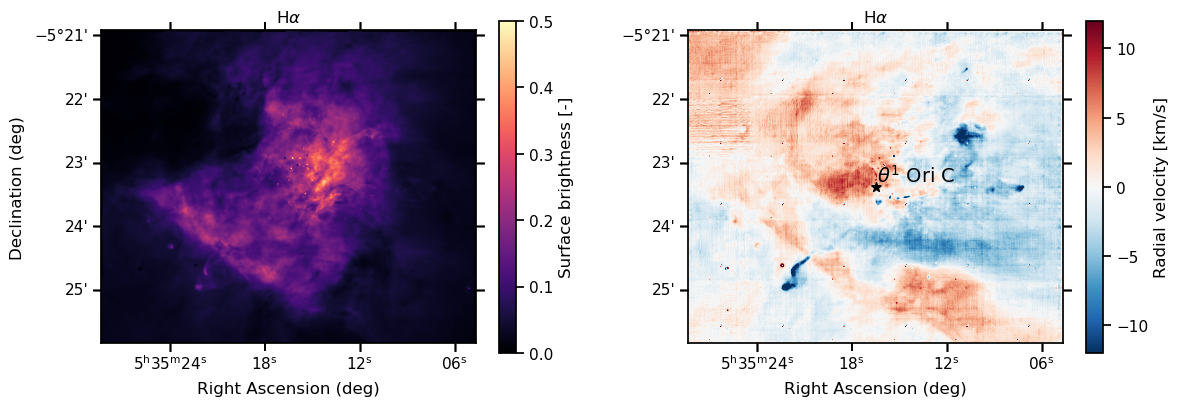
\includegraphics[width=6.5in]{figures/H_I-6563.png}\par
 \caption{
 Two-dimensional map of the integrated intensity (surface brightness) and the  velocity of the \halpha\ line for the Orion Nebula. 
 North is up and East is to the left.
 }
\label{fig:H_I-6563_maps}
\end{figure*}


\section{Plane-of-sky velocity fluctuations}\label{sec:met}

The overall amplitude of the plane-of-sky velocity fluctuations can be characterized by a dispersion, \(\sigma\pos\), defined as:

\begin{equation}
  \label{eq:sig-pos}
  \sigma^2\pos =
  \left\langle 
  \bigl[ V_c (\xx_i) -\langle V_ c\rangle  \bigr]^2
  \right \rangle ,
\end{equation}
where the average is performed over all observed points \(i\)
in a given map.
Note that \(\sigma\pos\) is also the RMS width of
the probability density function (PDF) of \(V_c\).

\begin{figure*}
 \centering
 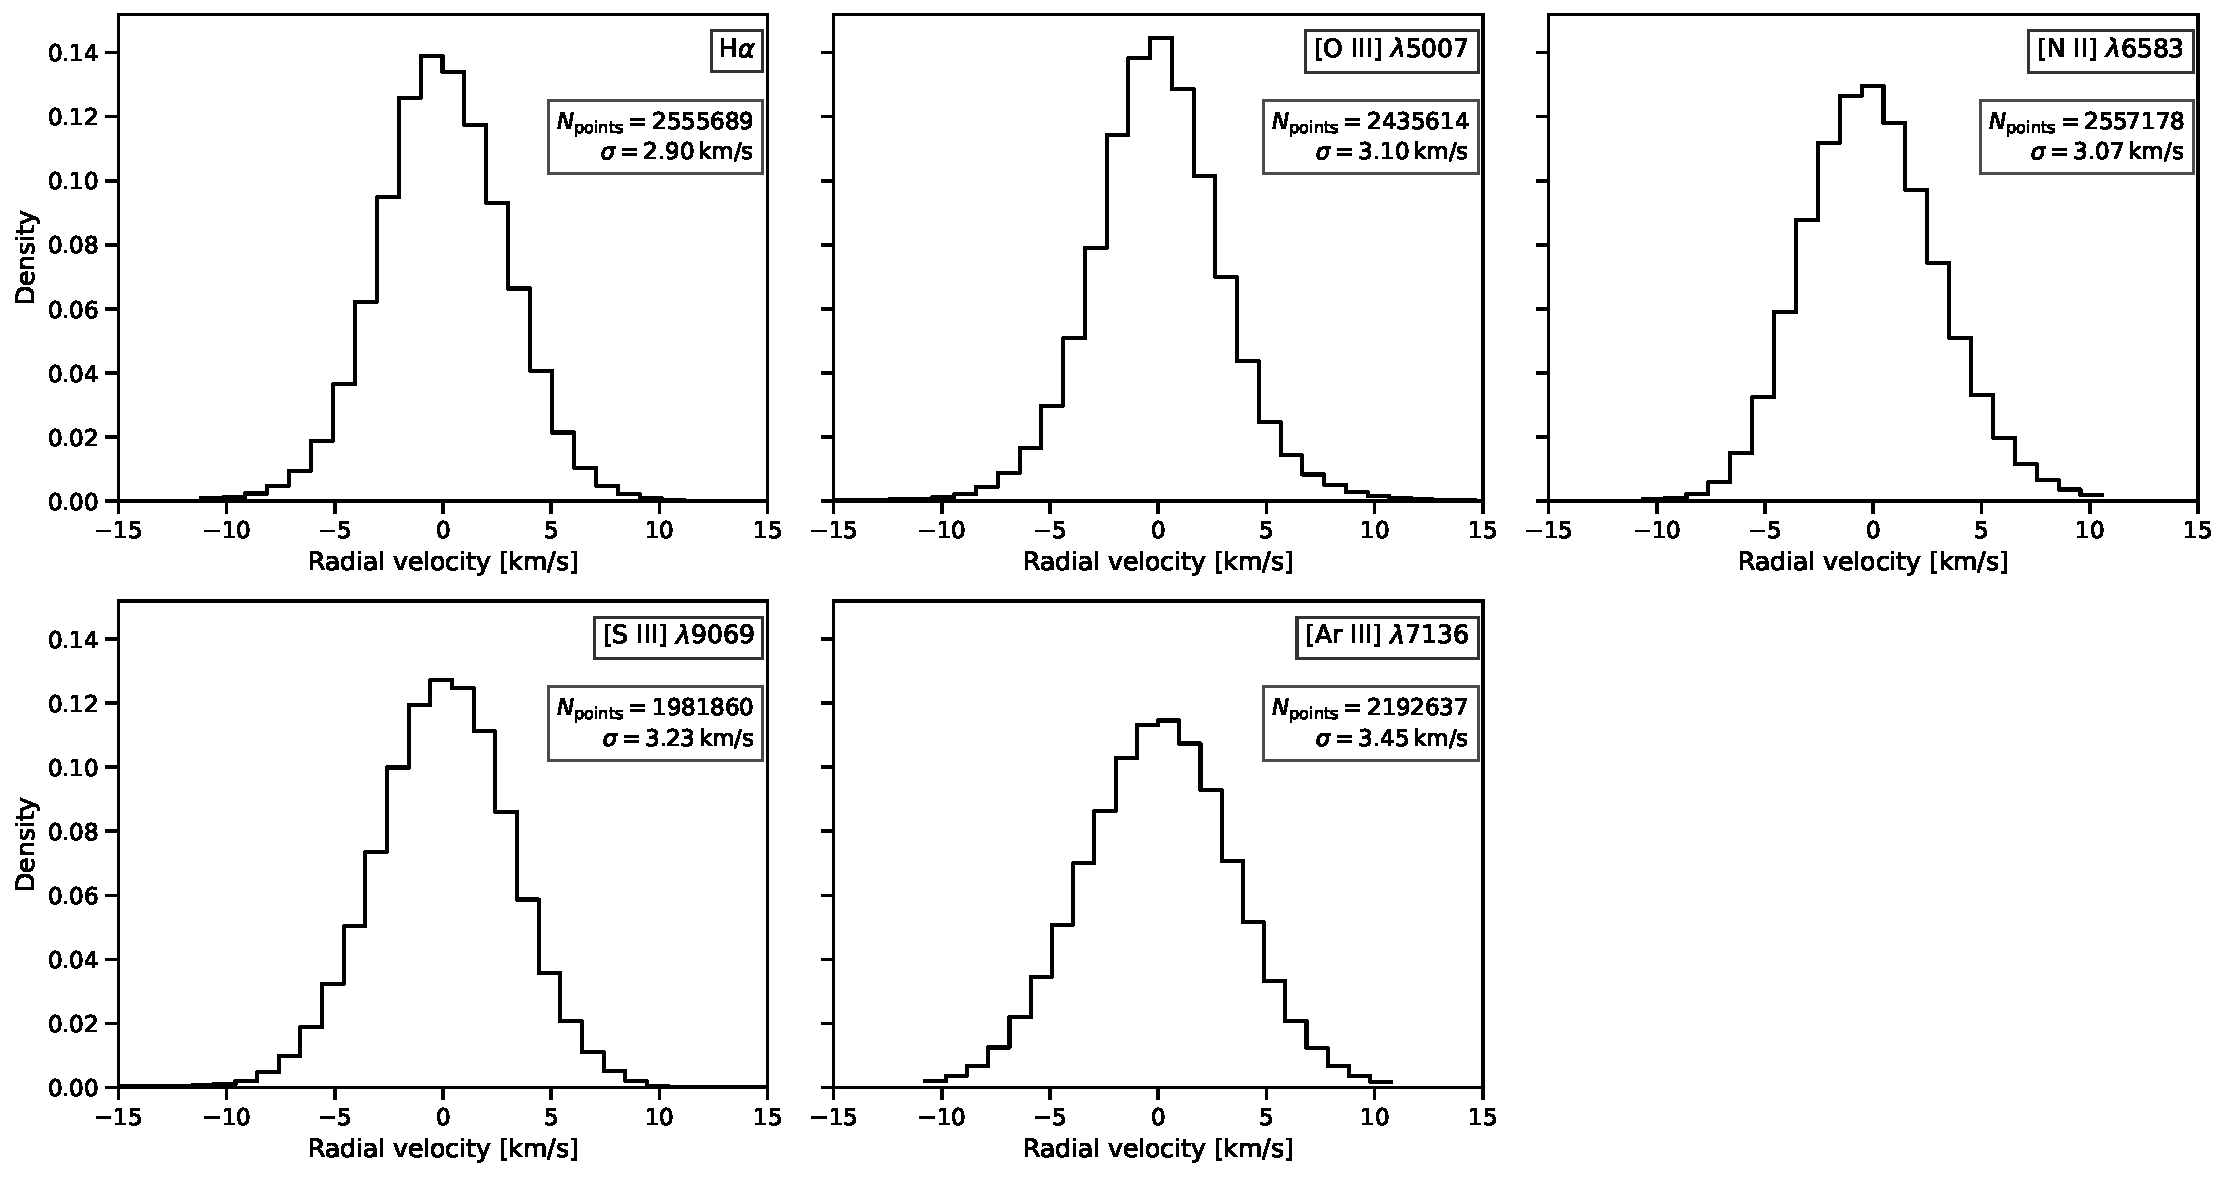
\includegraphics[width=5in]{figures/pdfs}\par
 \caption{
   Histograms of the plane-of-sky centroid velocities for different emission lines.
   Each panel shows the fraction of the observed spatial points
   with a given velocity offset from the mean systemic velocity of each region.
   The RMS width \(\sigma\pos\) of each distribution is marked,
   as is the number of spatial points.
   The bin width is \SI{1}{km.s^{-1}}.
 }
\label{fig:pdfs}
\end{figure*}

\begin{figure*}
 \centering
 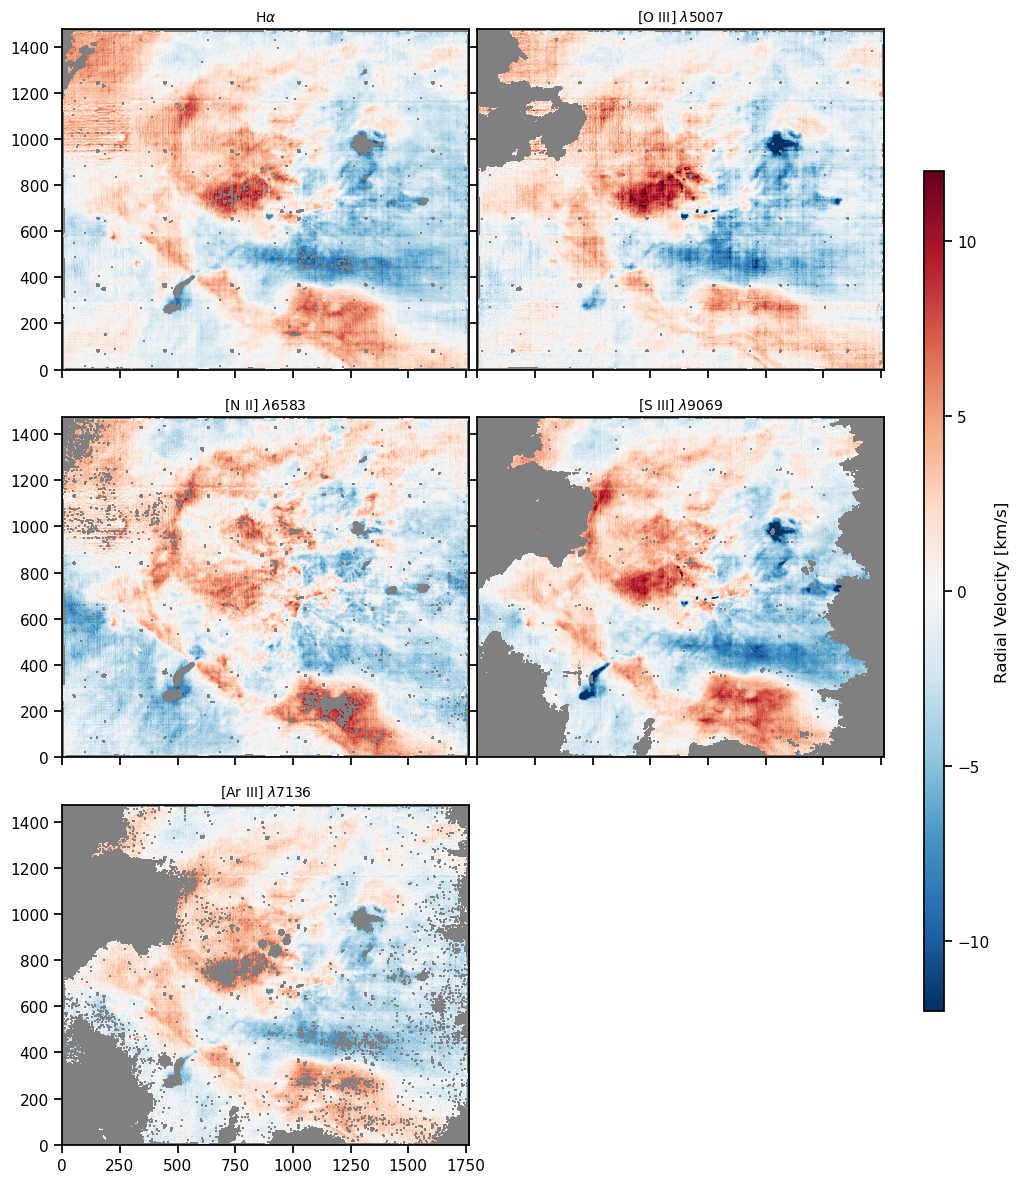
\includegraphics[width=6in]{figures/velocity_maps_shared_cbar_fixed}\par
 \caption{
 Two-dimensional velocity maps for different emission lines for the Orion nebula using MUSE/VLT observations. Each map has been masked to exclude all pixels with surface brightness below \(0.001\) times the peak or radial velocities greater than \(2\sigma_\text{pos}\). 
 }
\label{fig:figures/velocity_maps_shared_cbar_fixed.png}
\end{figure*}

\subsection{The binning proccedure}

To improve the signal-to-noise ratio (S/N) in regions of low surface brightness and to reduce the impact of small-scale noise fluctuations, we applied a spatial binning procedure to the original maps using the \texttt{tetrablock} Python package\footnote{\url{https://github.com/will-henney/tetrabloks}}.
This binning was performed by re-sampling the original data onto coarser grids, using binning factors of $2^1 = 2$, $2^2 = 4$, $2^3 = 8$, and $2^4 = 16$. 
Each binning level corresponds to averaging the velocity values within non-overlapping square regions of increasing size. 
The binning process not only enhances computational efficiency, but also allows us to test the robustness of the recovered turbulent parameters across different spatial resolutions. For consistency, all binned maps were later processed using the same masking criteria and structure function fitting method as applied to the original unbinned data.

Figure~\ref{fig:figures/Ha_maps_comparison} shows as an example of the binned velocity maps for the \halpha\ emission line.
The original map has a size of \(1 475 \times1765 \ \text{pixels}\) (see Fig.~\ref{fig:H_I-6563_maps}) which is reduced to a size of \(91 \times 109 \ \text{pixels}\) through a series of four iterations.
After applying the binning to each map, a mask was applied to exclude pixels with centroid velocity above \(2\sigma_\text{pos}\) and regions with normalized integrated intensity below \(0.001\).
Each iteration and the resulting velocity map is shown in the different panels of Fig.~\ref{fig:figures/Ha_maps_comparison}.

\begin{figure*}
 \centering
 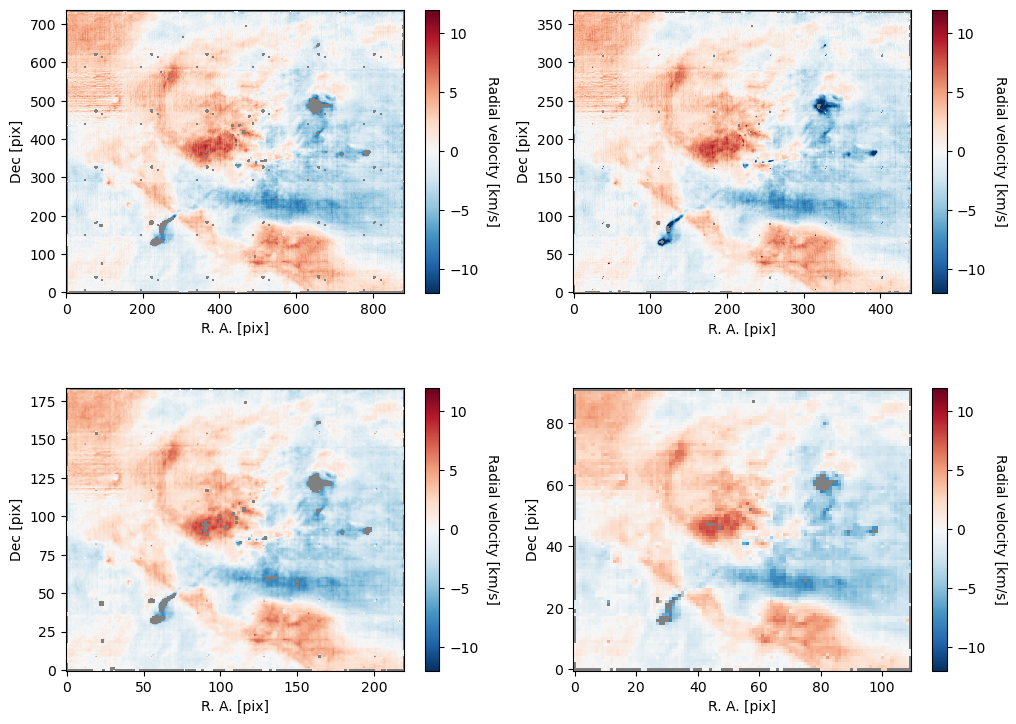
\includegraphics[width=6.5in]{figures/Ha_maps_comparison.png}\par
 \caption{
 Two-dimensional binned maps of the centroid velocity of the Orion nebula for the \halpha\ emission line. The size of each map are \(737 \times 882\), \(368\times 440\), \(183 \times 219\)  and \(91 \times 109 \ \text{pixels}\) which correspond to the bin sizes of $2$, $4$, $8$ and $16$ respectively. The same procedure of binning is applied to all emission lines mentioned in X.  
 }
\label{fig:figures/Ha_maps_comparison}
\end{figure*}

\subsection{The second-order structure function}
\label{sec:second-order-struct}

After the binning and masking of the maps we employ the second-order structure function, $B(r)$, which is a function of the scalar separation or lag, \(r\),
between two points on the plane of the sky:
%
\newcommand\Abs[1]{\vert #1\vert}
\begin{equation}\label{eq:Br}
  B(r) = \left\langle 
  \bigl[
  V_{c}(\xx_j) - V_{c}(\xx_i)
  \bigr]^{2} \right \rangle_{\Abs{\xx_j - \xx_i\!} \ \approx \ r} \ .
\end{equation}

The averaging is performed over all pairs of points
\((i, j)\)
whose scalar separation \(\Abs{\xx_j - \xx_i}\) is close to \(r\),
irrespective of the orientation of the separation vector.
In practice, we achieve this by binning the separations with a constant
logarithmic width of \SI{0.05}{dex}.

We will also employ the related quantity of the
normalized spatial autocovariance or autocorrelation function:
\begin{equation}
  \label{eq:autocovar}
  C(r) = \frac{1}{\sigma^2\pos}\left\langle 
  \bigl[
  V_{c}(\xx_j) \  V_{c}(\xx_i)
  \bigr] \right \rangle_{\Abs{\xx_j - \xx_i\!} \ \approx \ r} \ .
\end{equation}
If the fluctuations are perfectly spatially homogeneous, then the
two quantities are related \citep{1984ApJ...277..556S} as:
\begin{equation}\label{eq:functional}
  B(r) = 2\sigma^2\pos \bigl[   1 - C(r)\bigr] .
\end{equation}

%A common property of homogeneous fluctuating velocity fields is that neighboring points tend to have similar velocities (\(C(r) \approx 1\) for small \(r\)), whereas points that are far apart may have very different velocities (\(C(r) \ll 1\) for large \(r\)).
%The value of the separation that corresponds to the transition between these two regimes is called the correlation length, \(r_0\).
%In the simplest case, two points separated by \(r \gg r_0\) have totally uncorrelated velocities in the sense that knowledge of the velocity at the first point is of no help in predicting the velocity at the second point.
%At scales smaller than \(r_0\), the fluctuations often show a power-law behavior as a function of \(r\).

%In order to capture these two behaviors,

We  propose the following idealized 2-parameter model
for the autocorrelation function:
%
\begin{equation}\label{eq:new-correlation-form}
  C\model(r;\ r_0, m) = 2^{- \left( r/r_0 \right)^m} 
\end{equation}
%
in which \(r_{0}\)\ is the correlation length (see above)
and \(m\) is the power-law slope at small scales.
This is constructed so that \(C\model(r) = 1/2\) at \(r = r_0\),
while the exponential form ensures that \(C(r)\) rapidly approaches zero
for larger separations.
We assume the validity of equation~\eqref{eq:functional} to determine the structure function
from this model autocorrelation function:
\begin{equation}
  \label{eq:model-strucfunc-ideal}
  B\model(r) = 2\sigma^2\pos \left[
    1 - 2^{- \left( r/r_0 \right)^m} 
  \right]
\end{equation}
This has the following properties:
\begin{enumerate}[1.]
 \item Small scales: \(B\model(r) \propto r^m\) for \(r \ll r_0\);
 \item Correlation scale: \(B\model(r_0) = \sigma\pos^2\);
 \item Large scales: \(B\model(r) \to 2 \sigma\pos^2\) for \(r \gg r_0\).
 \end{enumerate}

Then, by combining both the effects of seeing $S(r)$ and noise $B\noise$ yields the corrected model structure function:
\begin{equation}
  \tilde{B}\model(r) = B\model(r) \,  S(r) + B\noise
  \label{eq:sf-functional}
\end{equation}


\section{Results}\label{sec:results}

In this section we present the turbulent paramaters and confidence intervals obtained through the fitting of the equation~\eqref{eq:sf-functional} to the observed structure function computed for each of the original masked maps and binned maps.
The posterior distributions of model parameters that are consistent with the observations for each emission line are estimated using Markov Chain Monte Carlo (MCMC) ensemble sampling \citep{2010CAMCS...5...65G} as implemented in the \texttt{emcee} Python library \citep{2013PASP..125..306F}.
The Table~\ref{tab:parameter-ranges} shows the uniform prior distribution that is assumed between upper and lower bounds for each parameter.


\begin{table}
  \centering
  \caption{Bounds of allowed values for parameters in model fits}
  \label{tab:parameter-ranges}
  \newlength\partabwidth
  \setlength\partabwidth{0.8\linewidth}
  \begin{tabular*}{\partabwidth}{
    l @{\extracolsep{\fill}}
    r 
    r
    }
    \toprule
    Parameter & Lower & Upper\\
    \midrule
    \(\sigma^2\) & \(0.25\, \max [B\obs]\)& \(2\, \max [B\obs]\)\\
    \(r_0\) & \(0.01\, L\) & \(2\, L\)\\
    \(m\) & \(0.5\) & \(2.0\) \\
    \(s_0\) & \SI{0.1}{arcsec}& \SI{1.5}{arcsec}\\
    \(B\noise\) & \(0\) & \(3\, \min [B\obs]\) \\
    \bottomrule
    \multicolumn{3}{@{}p{\partabwidth}@{}}{
    Note: \(\max[B\obs]\) and \(\min[B\obs]\) are over all bins in the observed structure function with \(r < L/2\).
    }
  \end{tabular*}
\end{table}


\subsection{Representative Case Study: \halpha\ and [ArIII] emission lines}\label{sec:discussion}

First, we present the results for the \halpha\ and [ArIII] emissiones lines.
Since they correspond to the brightest and faintest line, respectively, they are used to shows the effects of masking and binning in the structure function.
Then we apply the same analysis to the remaining lines in the following section.

Table~\ref{tab:results_MUSE_Ha} shows the best-fit values for the model parameters with  with 95\% credibility range for the \halpha\ line. 
The first column has the value for the binning size used in each map before computing the structure function.
The nuiscance values like the noise and seeing (in RMS and FWHM) are shown in columns three, four and ten.
The turbulent parameter are shown in columns two, six and seven.
Finally, columns eight and nine show the quotients $L/r_0$ and $s_0/r_0$, where $L$ is the observational box lenght, which are used for a sanity check of the results.

The solid markers (and different colors) in Figure~\ref{fig:figures/bin comparison} show the results of applying Equation~\eqref{eq:Br} to the masked \halpha\ and [ArIII] velocity maps (left and right panels, respectively), as shown in Figure~\ref{fig:figures/velocity_maps_shared_cbar_fixed} and the corresponding binned maps in Figure~\ref{fig:figures/Ha_maps_comparison}.

In Figure~\ref{fig:figures/bin comparison}, the strucutre function of each map is represented using different marker symbols.  
For the non-binned \halpha\ observed structure function (circles), the absence of a clear power-law behavior is evident, as much of the structure in the velocity fluctuations at small scales is buried beneath the instrumental noise.  
This result is consistent with the findings previously reported by \citet{2016MNRAS.455.4057M}, see their Figure~12.
The structure functions for the binned maps are also shown in Figure~\ref{fig:figures/bin comparison}, as indicated in the legend.  
It is evident that small-scale structure in the velocity field is progressively recovered as the bin size increases, as reflected in the emergence of a clear power-law behavior in each function.  
While smoothing helps reduce the impact of instrumental noise, high binning factors appear to be the most effective, at least in this case, at preserving the turbulent cascade while suppressing noise sufficiently to allow the smallest spatial scales to be sampled.

While for the largest scales, since the \halpha\ mask presents the better concordance between the non-binned map and binned map, the behavior at large scales is mantained for all the samples.
In this case the downward hook is a representaion of tapered fluctuaciones where the intensity of the fluctuacions is reduced at the border of the observational box.

The dotted line corresponds to the heuristic model described in equation~\eqref{eq:model-strucfunc-ideal} and fitted using..., while the dashed lines represent the ideal model given in equation~\eqref{eq:sf-functional}.  
For the \halpha\ emission, we were able to fit the model to all structure functions. While the ideal second-order structure function agrees well with all binned maps, a noticeable discrepancy remains with the non-binned results.  
This discrepancy is attributed to the lack of small-scale structure in the non-binned velocity map, as previously discussed.
This is better seen in Table~\ref{tab:results_MUSE_Ha} where the value obtained for the instrumental noise, \( B_{\text{noise}} \), decrease from a value of \SI{40}{km.s^{-1}} to \SI{0.5}{km.s^{-1}}.

Though, each binning iteration reduces the instrumental noise, this smoothing is at the expense of increasing the observational seeing in each sample. 
This is seen in the change of the $s_0$ value changing from \SI{\sim 1}{\text{arsec}} for the non-binned map to a value \SI{\sim 6}{\text{arsec}}.
Therefore there is a limit to the binning procedure in which we can reproduce the small scale fluctuactions and confidently recover the turbulent parameters.

The Table~\ref{tab:results_MUSE_Ar} shows the best-fit model parameters and their confidence intervals for the [Ar III] emission line and their structure functions are shown in the right panel of Figure~\ref{fig:figures/bin comparison}.

In this case, we observe that the non-binned structure function is not as strongly affected by noise as in the case of the \halpha\ emission line. 
However, it still lacks a coherent shape that resembles a typical structure function.  
The reduced impact of noise compared to \halpha\ is due to the more aggressive masking applied to the non-binned [ArIII] map.  
Since the normalization criterion is based on the surface brightness of the \halpha\ emission, any fainter emission line undergoes more intense masking. 
This effect is evident in Figure~\ref{fig:figures/velocity_maps_shared_cbar_fixed}.
In this case the reduction in noise for the non-binned case to the binning of \num{16} is from \SI{10}{km.s^{-1}} to \SI{0.5}{km.s^{-1}}, while the seeing...

For the [ArIII] emission line, we observe a good overall agreement with the model described by equation~\eqref{eq:model-strucfunc-ideal}.  
This indicates that the turbulent parameters as the slope \(m\), \(\sigma\)\pos, and the correlation length \(r_0\), are consistently recovered across all maps, both binned and non-binned.

We also find that Equation~\eqref{eq:sf-functional} can be successfully fitted to all observed structure functions.  
This demonstrates not only the applicability of the binning procedure in recovering the turbulent cascade in a computationally efficient manner, but also the effectiveness of the model in equation~\eqref{eq:sf-functional} for extracting the relevant turbulent parameters under certain S/N conditions.
%, if the noise is less than...see appendix...

Regarding the large scales in the structure function of the [ArIII] emission line, we observe a transition in behavior, which goes from a periodic, oscillatory pattern in the non-binned map (albeit masked, as previously discussed) to a radial-gradient pattern in the binned maps, similar to what is observed in the \halpha\ case.  
This change is primarily driven by the masking applied to the binned maps, which consistently excludes pixels with values above \(2\sigma_{Vc}\) for each iteration, thereby altering the large-scale structure.  

This observation is significant, as it suggests that large-scale fluctuations may be line-dependent, which is consistent with the expected spatial distribution of different ions within the nebula.

\begingroup
\setlength{\tabcolsep}{6pt} % Default value: 6pt
\renewcommand{\arraystretch}{1.5} % Default value: 1
%% In Emacs we can use M-x align-current to align the table on the & symbols after editing
\begin{table*}
\begin{center}
  \caption{
    Best-fit model parameters and 95\% credibility intervals for fits to observed structure functions in the Orion core for the VLT MUSE \halpha\ line observations.
  }

%\begin{adjustbox}{width=1\textwidth}
  
  \begin{tabular}{l RRRRRR  @{\hspace{6\tabcolsep}} RRR}
    \toprule
Binning   & \sigma^2\pos            & B_{\text{noise}}       & s_0 (\text{RMS})       & r_0             & L        & m                   & L/r_0    & s_0 / r_0 & s_0 (\text{FWHM}) \\
         & [\si{km^2.s^{-2}}] & [\si{km^2.s^{-2}}]     & [\si{pc}]                 & [\si{pc}]              & [\si{pc}] & [-]                 & [-]   & [-]       & [\text{arcsec}]   \\
\midrule
None   & 95.46\PM{49.22}{58.05} & 42.410\PM{2.197}{0.895} & >0.0002 & 0.881\PM{0.383}{0.670}   & 0.64    & 0.78\PM{0.20}{0.10} & 0.72  & 0.0002   & >0.3  \\
2    & 7.84\PM{0.20}{0.16}  & 1.416\PM{0.093}{0.043}  & >0.001 & 0.066\PM{0.003}{0.002}  & 0.64    & 1.16\PM{0.03}{0.03} & 10  & 0.004   & >1.2\\
4    & 7.09\PM{0.13}{0.10}  & 1.049\PM{0.125}{0.076}  & >0.001 & 0.050\PM{0.001}{0.001} & 0.64    & 1.19\PM{0.04}{0.04} & 13  & 0.007   & >1.2 \\
8    & 6.34\PM{0.15}{0.07}  & 0.478\PM{0.126}{0.060}  & >0.0014 & 0.055\PM{0.001}{0.001} & 0.64    & 1.36\PM{0.04}{0.04} & 11   & 0.004      & >1.7  \\
16  & 8.12\PM{1.00}{0.31}  & >0.5 & >0.005 & 0.074\PM{0.008}{0.005} & 0.64    & 1.20\PM{0.06}{0.11} & 9   & 0.004      & >5.77  \\

  \bottomrule

\end{tabular}\label{tab:results_MUSE_Ha}
%\end{adjustbox}
\end{center}
\end{table*}
\endgroup


\begingroup
\setlength{\tabcolsep}{6pt} % Default value: 6pt
\renewcommand{\arraystretch}{1.5} % Default value: 1
%% In Emacs we can use M-x align-current to align the table on the & symbols after editing
\begin{table*}
\begin{center}
  \caption{
    Best-fit model parameters and 95\% credibility intervals for fits to observed structure functions in the Orion core for the VLT MUSE [ArIII] line observations.
  }

%\begin{adjustbox}{width=1\textwidth}
  
  \begin{tabular}{l RRRRRR  @{\hspace{6\tabcolsep}} RRR}
    \toprule
Binning   & \sigma^2\pos            & B_{\text{noise}}       & s_0 (\text{RMS})       & r_0             & L        & m                   & L/r_0    & s_0 / r_0 & s_0 (\text{FWHM}) \\
         & [\si{km^2.s^{-2}}] & [\si{km^2.s^{-2}}]     & [\si{pc}]                 & [\si{pc}]              & [\si{pc}] & [-]                 & [-]   & [-]       & [\text{arcsec}]   \\
\midrule
None & 8.62\PM{3.08}{0.54}  & 9.717\PM{0.339}{0.091}  & 0.0002\PM{0.0045}{-0.0001}  & 0.071\PM{0.039}{0.007}   & 0.64    & 1.10\PM{0.08}{0.24} & 9   & 0.0028   & 0.24\PM{5.36}{-0.08} \\
2    & 8.46\PM{1.90}{0.41}  & 5.122\PM{0.406}{0.059}  & 0.0002\PM{0.0045}{-0.0001} & 0.066\PM{0.019}{0.005} & 0.64    & 1.09\PM{0.06}{0.19} & 9   & 0.003   & 0.24\PM{5.29}{-0.09} \\
4    & 8.11\PM{1.26}{0.42}  & 2.101\PM{0.291}{0.201}  & 0.0011\PM{0.0033}{0.0008} & 0.068\PM{0.014}{0.005} & 0.64    & 1.09\PM{0.05}{0.14} & 9   & 0.016   & 1.32\PM{3.91}{1.00} \\
8    & 8.49\PM{0.94}{0.70}  & 0.952\PM{0.136}{0.385}  & 0.0034\PM{0.0014}{0.0030} & 0.070\PM{0.011}{0.006} & 0.64    & 1.05\PM{0.09}{0.10} & 9   & 0.049     & 4.04\PM{1.71}{3.52}  \\
16   &  8.50\PM{0.58}{0.83} & 0.574\PM{0.124}{0.527}  & 0.0050\PM{-0.0000}{0.0044} & 0.067\PM{0.009}{0.005} & 0.64    & 1.05\PM{0.13}{0.06} & 9   & 0.074      & 5.87\PM{-0.06}{5.17}  \\

  \bottomrule

\end{tabular}\label{tab:results_MUSE_Ar}
%\end{adjustbox}
\end{center}
\end{table*}
\endgroup



\begin{figure*}
 \centering
 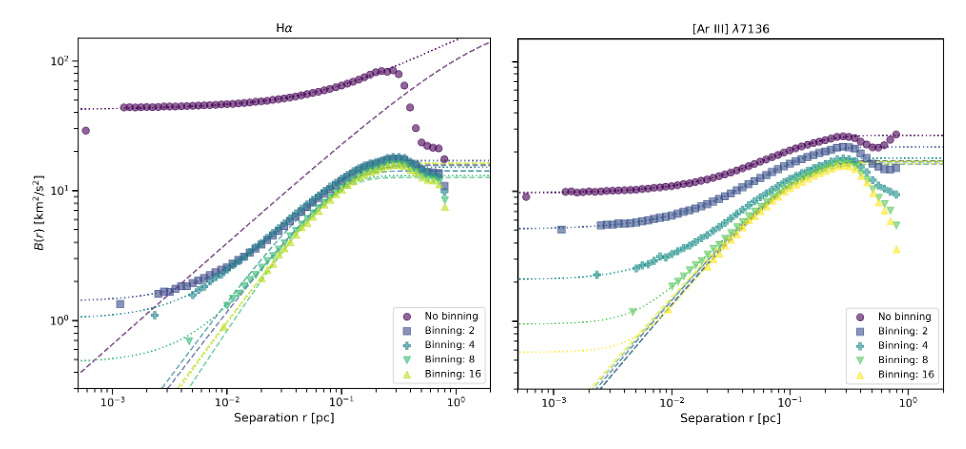
\includegraphics[width=6.5in]{figures/bin comparison.png}\par
 \caption{
 }
\label{fig:figures/bin comparison}
\end{figure*}

\begin{figure*}
  \centering
  \sffigggg{H_I-6563_mask_bin_4}{H_I-6563_mask_bin_4}{Ar_III-7136_mask_bin_4}{Ar_III-7136_mask_bin_4}
  \caption{ Results for binning 4
  }
  \label{fig:Orion_sf_1}
\end{figure*}

\subsection{Application to Additional Emission Lines}

Continue here...




\begin{figure*}
  \centering
  \sffigggg{O_III-5007_mask_bin_4}{O_III-5007_mask_bin_4}{O_III-4959_mask_bin_4}{O_III-4959_mask_bin_4}
  \caption{ Results for binning 4
  }
  \label{fig:Orion_sf_O}
\end{figure*}


\begin{figure*}
  \centering
  \sffigggg{N_II-6583_mask_bin_4}{N_II-6583_mask_bin_4}{N_II-6548_mask_bin_4}{N_II-6548_mask_bin_4}
  \caption{ Results for binning 4
  }
  \label{fig:Orion_sf_N}
\end{figure*}


\begin{figure*}
  \centering
  \sffigg{S_III-9069_mask_bin_4}{S_III-9069_mask_bin_4}
  \caption{ Results for binning 4
  }
  \label{fig:Orion_sf_S}
\end{figure*}

\section{Discussion}\label{sec:discussion}

\begingroup
\setlength{\tabcolsep}{6pt} % Default value: 6pt
\renewcommand{\arraystretch}{1.5} % Default value: 1
%% In Emacs we can use M-x align-current to align the table on the & symbols after editing
\begin{table*}
\begin{center}
  \caption{
    Best-fit model parameters and 95\% credibility intervals for fits to observed structure functions in the Orion core for the VLT MUSE (bin=4) observations.
  }

%\begin{adjustbox}{width=1\textwidth}
  
  \begin{tabular}{l RRRRRR  @{\hspace{6\tabcolsep}} RRR}
    \toprule
Line   & \sigma^2\pos            & B_{\text{noise}}       & s_0 (\text{RMS})       & r_0             & L        & m                   & L/r_0    & s_0 / r_0 & s_0 (\text{FWHM}) \\
         & [\si{km^2.s^{-2}}] & [\si{km^2.s^{-2}}]     & [\si{pc}]                 & [\si{pc}]              & [\si{pc}] & [-]                 & [-]   & [-]       & [\text{arcsec}]   \\
\midrule
H I 6563    & 7.09\PM{0.13}{0.10}  & 1.049\PM{0.125}{0.076}  & 0.0004\PM{0.0007}{0.0002} & 0.050\PM{0.001}{0.001} & 0.64    & 1.19\PM{0.04}{0.04} & 13  & 0.007   & 0.43\PM{0.78}{0.18} \\
O III 5007  &  8.77\PM{1.10}{0.61} & 1.113\PM{0.199}{0.122}  & 0.0005\PM{0.0012}{0.0002} & 0.083\PM{0.016}{0.008} & 0.64    & 1.03\PM{0.05}{0.06} & 8   & 0.005   & 0.54\PM{1.37}{0.28}  \\
O III 4959  & 8.79\PM{1.53}{0.67}  & 2.552\PM{0.339}{0.168} & 0.0005\PM{0.0025}{0.0002} & 0.082\PM{0.022}{0.009} & 0.64    & 1.03\PM{0.07}{0.10}  & 8   & 0.005   & 0.57\PM{2.94}{0.29}  \\
N II 6583   & 8.44\PM{0.87}{0.50}  & 0.727\PM{0.319}{0.163}  & 0.0005\PM{0.0013}{0.0002} & 0.064\PM{0.012}{0.006} & 0.64    & 0.93\PM{0.05}{0.06} & 10  & 0.007   & 0.55\PM{1.52}{0.28} \\
N II 6548   & 9.23\PM{1.89}{0.76} & 1.546\PM{0.458}{0.220}  & 0.0005\PM{0.0020}{0.0002} & 0.078\PM{0.031}{0.009} & 0.64    & 0.89\PM{0.06}{0.09}  & 8   & 0.005   & 0.55\PM{2.40}{0.27} \\
S III 9069  & 8.94\PM{0.70}{0.42}  & 0.601\PM{0.181}{0.076}  & 0.0004\PM{0.0013}{0.0002} & 0.072\PM{0.008}{0.005} & 0.64    & 1.11\PM{0.04}{0.05} & 9   & 0.006   & 0.52\PM{1.54}{0.25}  \\
Ar III 7136 & 8.11\PM{1.26}{0.42}  & 2.101\PM{0.291}{0.201}  & 0.0011\PM{0.0033}{0.0008} & 0.068\PM{0.014}{0.005} & 0.64    & 1.09\PM{0.05}{0.14} & 9   & 0.016   & 1.32\PM{3.91}{1.00} \\
  \bottomrule

\end{tabular}\label{tab:results_KPNO}
%\end{adjustbox}
\end{center}
\end{table*}
\endgroup


\begingroup
\setlength{\tabcolsep}{6pt} % Default value: 6pt
\renewcommand{\arraystretch}{1.5} % Default value: 1
%% In Emacs we can use M-x align-current to align the table on the & symbols after editing
\begin{table*}
\begin{center}
  \caption{
    Best-fit model parameters and 95\% credibility intervals for fits to observed structure functions in the Orion core for the KPNO echelle observations.
  }

%\begin{adjustbox}{width=1\textwidth}
  
  \begin{tabular}{l RRRRRR  @{\hspace{6\tabcolsep}} RRR}
    \toprule
Element   & \sigma^2\pos            & B_{\text{noise}}       & s_0 (\text{RMS})          & r_0                    & L         & m                   & L/r_0 & s_0 / r_0 & s_0 (\text{FWHM}) \\
         & [\si{km^2.s^{-2}}] & [\si{km^2.s^{-2}}]     & [\si{pc}]                 & [\si{pc}]              & [\si{pc}] & [-]                 & [-]   & [-]       & [\text{arcsec}]   \\
\midrule
H   & 12.0\PM{0.5}{0.5}        & 0.025\PM{0.003}{0.002} & 0.0016\PM{0.0001}{0.0001} & 0.068\PM{0.003}{0.002} & 0.5       & 1.07\PM{0.02}{0.02} & 7     & 0.03      & 2.4\PM{0.4}{0.3}  \\
O   & 11.0\PM{0.5}{0.4}        & 0.025\PM{0.004}{0.004} & 0.0018\PM{0.0002}{0.0002} & 0.061\PM{0.004}{0.003} & 0.45       & 1.18\PM{0.03}{0.04} & 7.4     & 0.03      & 2.13\PM{0.3}{0.2}  \\
N    & 12\PM{2}{1}        & 0.028\PM{0.011}{0.014} & 0.0036\PM{0.0009}{0.0004} & 0.050\PM{0.030}{0.006} & 0.45       & 0.66\PM{0.06}{0.11} & 9     & 0.07      & 2.13\PM{0.3}{0.2}  \\
S   & 6.35\PM{0.23}{0.84}        & 0.031\PM{0.02}{0.01} & 0.0030\PM{0.0001}{0.000} & 0.045\PM{0.05}{0.01} & 0.35       & 0.62\PM{0.06}{0.11} &  7.5    & 0.03      & 3.2 \PM{1.0}{0.5}  \\
  \bottomrule

\end{tabular}\label{tab:results_KPNO}
%\end{adjustbox}
\end{center}
\end{table*}
\endgroup



\section{Summary}\label{sec:summary}


\section*{Acknowledgements}

\section*{Data availability statement}
\label{sec:data-avail-stat}
All data and accompanying analysis programs used in this paper are available
from the github repository \url{https://github.com/JavGVastro/orion_muse}.

\bibliographystyle{mnras}
\bibliography{turb-refs}

%\clearpage

%\clearpage

%%%%%%%%%%%%%%%%%%%%%%%%%%%%%%%%%%%%%%%%%%%%%%%%%%
%%%%%%%%%%%%%%%%% APPENDICES %%%%%%%%%%%%%%%%%%%%%
%%%%%%%%%%%%%%%%%%%%%%%%%%%%%%%%%%%%%%%%%%%%%%%%%%

\appendix

\section{Multiple emission line maps} \label{apex:multiple_lines_maps}

\begin{figure*}
 \centering
 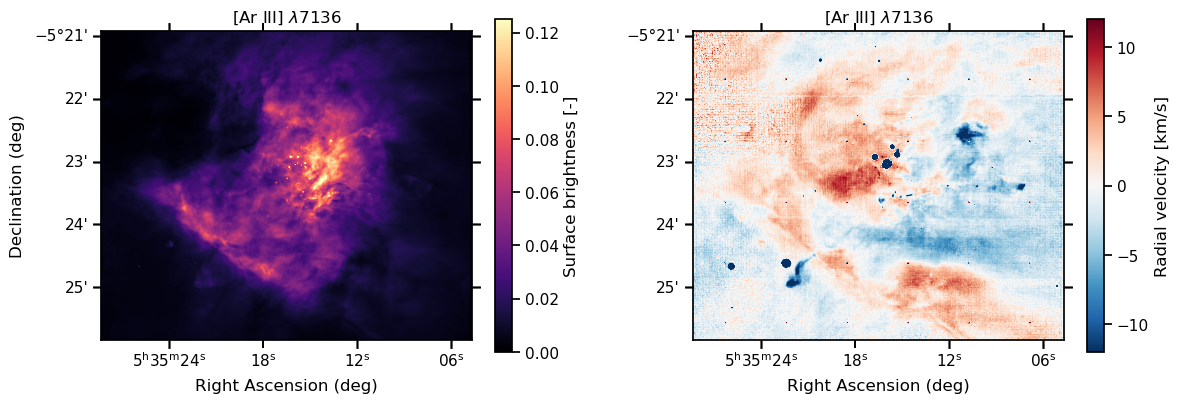
\includegraphics[width=6.5in]{figures/Ar_III-7136.png}\par
 \caption{
 Two-dimensional map of the integrated intensity (surface brightness) and the  velocity of the [ArIII] line for the Orion Nebula. 
 North is up and East is to the left.
 }
\label{fig:Ar_maps}
\end{figure*}


\section{Results for different binning iterations} \label{apex:multiple_lines_results}

Here we show tables \ref{tab:results_MUSE_O} - \ref{tab:results_MUSE_S}

\begingroup
\setlength{\tabcolsep}{6pt} % Default value: 6pt
\renewcommand{\arraystretch}{1.5} % Default value: 1
%% In Emacs we can use M-x align-current to align the table on the & symbols after editing
\begin{table*}
\begin{center}
  \caption{
    Best-fit model parameters and 95\% credibility intervals for fits to observed structure functions in the Orion core for the VLT MUSE [OIII] 5007 line observations.
  }

%\begin{adjustbox}{width=1\textwidth}
  
  \begin{tabular}{l RRRRRR  @{\hspace{6\tabcolsep}} RRR}
    \toprule
Binning   & \sigma^2\pos            & B_{\text{noise}}       & s_0 (\text{RMS})       & r_0             & L        & m                   & L/r_0    & s_0 / r_0 & s_0 (\text{FWHM}) \\
         & [\si{km^2.s^{-2}}] & [\si{km^2.s^{-2}}]     & [\si{pc}]                 & [\si{pc}]              & [\si{pc}] & [-]                 & [-]   & [-]       & [\text{arcsec}]   \\
\midrule
None  & 9.33\PM{1.90}{0.79} & 6.322\PM{0.232}{0.117} & 0.0002\PM{0.0015}{0.0000}     & 0.081\PM{0.028}{0.010}   & 0.64    & 1.01\PM{0.07}{0.10} & 8   & 0.0026   & 0.26\PM{1.73}{0.00}  \\
2  & 8.74\PM{1.12}{0.61} & 2.641\PM{0.188}{0.089} & 0.0003\PM{0.0013}{0.0001} & 0.081\PM{0.016}{0.008}    & 0.64    & 1.05\PM{0.06}{0.07} & 8   & 0.004   & 0.38\PM{1.51}{0.12}  \\
4  &  8.77\PM{1.10}{0.61} & 1.113\PM{0.199}{0.122}  & 0.0005\PM{0.0012}{0.0002} & 0.083\PM{0.016}{0.008} & 0.64    & 1.03\PM{0.05}{0.06} & 8   & 0.005   & 0.54\PM{1.37}{0.28}  \\
8  &  8.04\PM{1.09}{0.47} & 0.530\PM{0.304}{0.133}  & 0.0006\PM{0.0029}{0.0004} & 0.081\PM{0.015}{0.006} & 0.64    & 1.09\PM{0.05}{0.09} & 8   & 0.008    & 0.77\PM{3.43}{0.46}  \\
16  & 8.25\PM{0.72}{0.77}  & 0.467\PM{0.113}{0.430}  & 0.0043\PM{0.0006}{0.0039}  & 0.080\PM{0.011}{0.007} & 0.64    & 1.10\PM{0.10}{0.07} & 8   & 0.053      & 5.09\PM{0.68}{4.61}  \\


  \bottomrule

\end{tabular}\label{tab:results_MUSE_O}
%\end{adjustbox}
\end{center}
\end{table*}
\endgroup

\begingroup
\setlength{\tabcolsep}{6pt} % Default value: 6pt
\renewcommand{\arraystretch}{1.5} % Default value: 1
%% In Emacs we can use M-x align-current to align the table on the & symbols after editing
\begin{table*}
\begin{center}
  \caption{
    Best-fit model parameters and 95\% credibility intervals for fits to observed structure functions in the Orion core for the VLT MUSE [OIII] 4959 line observations.
  }

%\begin{adjustbox}{width=1\textwidth}
  
  \begin{tabular}{l RRRRRR  @{\hspace{6\tabcolsep}} RRR}
    \toprule
Binning   & \sigma^2\pos            & B_{\text{noise}}       & s_0 (\text{RMS})       & r_0             & L        & m                   & L/r_0    & s_0 / r_0 & s_0 (\text{FWHM}) \\
         & [\si{km^2.s^{-2}}] & [\si{km^2.s^{-2}}]     & [\si{pc}]                 & [\si{pc}]              & [\si{pc}] & [-]                 & [-]   & [-]       & [\text{arcsec}]   \\
\midrule
None  & 10.17\PM{21.51}{1.09}  & 13.392\PM{0.412}{0.282} & 0.0003\PM{0.0040}{0.0000} & 0.084\PM{0.567}{0.013}   & 0.64    &   0.98\PM{0.10}{0.29}  & 8   & 0.0031   & 0.31\PM{4.76}{0.04}  \\
2  & 8.70\PM{2.03}{0.68}  & 6.393\PM{0.322}{0.158} & 0.0004\PM{0.0033}{0.0001} & 0.079\PM{0.029}{0.009}   & 0.64    & 1.08\PM{0.08}{0.14}  & 8   & 0.004   & 0.42\PM{3.91}{0.14}  \\
4  & 8.79\PM{1.53}{0.67}  & 2.552\PM{0.339}{0.168} & 0.0005\PM{0.0025}{0.0002} & 0.082\PM{0.022}{0.009} & 0.64    & 1.03\PM{0.07}{0.10}  & 8   & 0.005   & 0.57\PM{2.94}{0.29}  \\
8  & 8.65\PM{1.43}{0.58}  & 0.927\PM{0.382}{0.191}  & 0.0007\PM{0.0032}{0.0004} & 0.083\PM{0.020}{0.007} & 0.64    & 1.06\PM{0.06}{0.10} & 8   & 0.008      & 0.81\PM{3.83}{0.51}  \\
16   & 8.16\PM{1.04}{0.64}  & 0.530\PM{0.203}{0.451}  & 0.0032\PM{0.0016}{0.0029}  & 0.082\PM{0.014}{0.007} & 0.64    & 1.11\PM{0.08}{0.10} & 8   & 0.039      & 3.80\PM{1.94}{3.41}  \\



  \bottomrule

\end{tabular}\label{tab:results_MUSE_O4959}
%\end{adjustbox}
\end{center}
\end{table*}
\endgroup

\begingroup
\setlength{\tabcolsep}{6pt} % Default value: 6pt
\renewcommand{\arraystretch}{1.5} % Default value: 1
%% In Emacs we can use M-x align-current to align the table on the & symbols after editing
\begin{table*}
\begin{center}
  \caption{
    Best-fit model parameters and 95\% credibility intervals for fits to observed structure functions in the Orion core for the VLT MUSE [NII] 6583 line observations.
  }

%\begin{adjustbox}{width=1\textwidth}
  
  \begin{tabular}{l RRRRRR  @{\hspace{6\tabcolsep}} RRR}
    \toprule
Binning   & \sigma^2\pos            & B_{\text{noise}}       & s_0 (\text{RMS})       & r_0             & L        & m                   & L/r_0    & s_0 / r_0 & s_0 (\text{FWHM}) \\
         & [\si{km^2.s^{-2}}] & [\si{km^2.s^{-2}}]     & [\si{pc}]                 & [\si{pc}]              & [\si{pc}] & [-]                 & [-]   & [-]       & [\text{arcsec}]   \\
\midrule
None   & 8.42\PM{1.44}{0.68}  & 4.861\PM{0.317}{0.106} & 0.0002\PM{0.0014}{-0.0000}   & 0.066\PM{0.023}{0.008}   & 0.64    &  0.89\PM{0.07}{0.08} & 10  & 0.0030   & 0.24\PM{1.63}{-0.01} \\
2   & 8.83\PM{1.02}{0.59}  & 1.964\PM{0.326}{0.123} & 0.0003\PM{0.0011}{0.0001}   & 0.064\PM{0.014}{0.007}   & 0.64    & 0.89\PM{0.05}{0.06} & 10  & 0.005   & 0.37\PM{1.31}{0.12} \\
4   & 8.44\PM{0.87}{0.50}  & 0.727\PM{0.319}{0.163}  & 0.0005\PM{0.0013}{0.0002}  & 0.064\PM{0.012}{0.006} & 0.64    & 0.93\PM{0.05}{0.06} & 10  & 0.007   & 0.55\PM{1.52}{0.28} \\
8   & 8.43\PM{1.57}{0.61}  & 0.580\PM{0.208}{0.493}  & 0.0026\PM{0.0021}{0.0022}  & 0.065\PM{0.020}{0.007} & 0.64    & 0.94\PM{0.07}{0.14} & 10  & 0.039      & 3.06\PM{2.52}{2.62}  \\
16   & 8.56\PM{0.99}{0.90}  & 0.444\PM{0.159}{0.415}  & 0.0050\PM{-0.0000}{0.0031} & 0.066\PM{0.015}{0.008} & 0.64    & 0.90\PM{0.13}{0.08} & 10  & 0.075      & 5.87\PM{-0.04}{3.69}  \\



  \bottomrule

\end{tabular}\label{tab:results_MUSE_N}
%\end{adjustbox}
\end{center}
\end{table*}
\endgroup

\begingroup
\setlength{\tabcolsep}{6pt} % Default value: 6pt
\renewcommand{\arraystretch}{1.5} % Default value: 1
%% In Emacs we can use M-x align-current to align the table on the & symbols after editing
\begin{table*}
\begin{center}
  \caption{
    Best-fit model parameters and 95\% credibility intervals for fits to observed structure functions in the Orion core for the VLT MUSE [NII] 6548 line observations.
  }

%\begin{adjustbox}{width=1\textwidth}
  
  \begin{tabular}{l RRRRRR  @{\hspace{6\tabcolsep}} RRR}
    \toprule
Binning   & \sigma^2\pos            & B_{\text{noise}}       & s_0 (\text{RMS})       & r_0             & L        & m                   & L/r_0    & s_0 / r_0 & s_0 (\text{FWHM}) \\
         & [\si{km^2.s^{-2}}] & [\si{km^2.s^{-2}}]     & [\si{pc}]                 & [\si{pc}]              & [\si{pc}] & [-]                 & [-]   & [-]       & [\text{arcsec}]   \\
\midrule
None   & 14.53\PM{28.55}{1.77} & 6.159\PM{0.825}{0.155} & 0.0002\PM{0.0025}{-0.0000}  & 0.104\PM{1.036}{0.021}   & 0.64    & 0.72\PM{0.06}{0.15}  & 6   & 0.0019   & 0.24\PM{2.96}{-0.03} \\
2   & 9.07\PM{2.00}{0.76} & 4.007\PM{0.439}{0.185} & 0.0004\PM{0.0021}{0.0001} & 0.071\PM{0.032}{0.009}    & 0.64    & 0.89\PM{0.07}{0.10}  & 9   & 0.005   & 0.42\PM{2.47}{0.16} \\
4   & 9.23\PM{1.89}{0.76} & 1.546\PM{0.458}{0.220}  & 0.0005\PM{0.0020}{0.0002} & 0.078\PM{0.031}{0.009} & 0.64    & 0.89\PM{0.06}{0.09}  & 8   & 0.005   & 0.55\PM{2.40}{0.27} \\
8   & 9.16\PM{2.48}{0.68}  & 0.749\PM{0.318}{0.549}  & 0.0020\PM{0.0026}{0.0017} & 0.077\PM{0.040}{0.009} & 0.64    & 0.92\PM{0.06}{0.14} & 8   & 0.025     & 2.31\PM{3.08}{1.97}  \\
16 & 8.91\PM{2.23}{0.70}  & 0.000\PM{0.871}{-0.026} & 0.0011\PM{0.0039}{0.0002}  & 0.074\PM{0.035}{0.007} & 0.64    & 0.93\PM{0.08}{0.14} & 9   & 0.014      & 1.25\PM{4.57}{0.24}  \\




  \bottomrule

\end{tabular}\label{tab:results_MUSE_N6548}
%\end{adjustbox}
\end{center}
\end{table*}
\endgroup

\begingroup
\setlength{\tabcolsep}{6pt} % Default value: 6pt
\renewcommand{\arraystretch}{1.5} % Default value: 1
%% In Emacs we can use M-x align-current to align the table on the & symbols after editing
\begin{table*}
\begin{center}
  \caption{
    Best-fit model parameters and 95\% credibility intervals for fits to observed structure functions in the Orion core for the VLT MUSE [SIII] 9069 line observations.
  }

%\begin{adjustbox}{width=1\textwidth}
  
  \begin{tabular}{l RRRRRR  @{\hspace{6\tabcolsep}} RRR}
    \toprule
Binning   & \sigma^2\pos            & B_{\text{noise}}       & s_0 (\text{RMS})       & r_0             & L        & m                   & L/r_0    & s_0 / r_0 & s_0 (\text{FWHM}) \\
         & [\si{km^2.s^{-2}}] & [\si{km^2.s^{-2}}]     & [\si{pc}]                 & [\si{pc}]              & [\si{pc}] & [-]                 & [-]   & [-]       & [\text{arcsec}]   \\
\midrule
None  & 11.29\PM{0.82}{0.55}  & 2.928\PM{0.214}{0.057}  & 0.0002\PM{0.0008}{-0.0000} & 0.060\PM{0.007}{0.005}   & 0.64    & 1.00\PM{0.04}{0.04} & 10   & 0.0033   & 0.24\PM{0.90}{-0.01} \\
2  & 9.27\PM{0.80}{0.49}  & 1.702\PM{0.192}{0.059}  & 0.0003\PM{0.0012}{0.0001} & 0.071\PM{0.010}{0.005}  & 0.64    & 1.07\PM{0.05}{0.05} & 9   & 0.004   & 0.33\PM{1.46}{0.07} \\
4   & 8.94\PM{0.70}{0.42}  & 0.601\PM{0.181}{0.076}  & 0.0004\PM{0.0013}{0.0002} & 0.072\PM{0.008}{0.005} & 0.64    & 1.11\PM{0.04}{0.05} & 9   & 0.006   & 0.52\PM{1.54}{0.25}  \\
8  & 8.93\PM{0.94}{0.45}  & 0.402\PM{0.192}{0.247}  & 0.0017\PM{0.0022}{0.0014} & 0.070\PM{0.009}{0.005} & 0.64    & 1.13\PM{0.05}{0.10} & 9   & 0.023     & 1.97\PM{2.66}{1.66}  \\
16   & 9.27\PM{0.50}{0.90}  & 0.698\PM{0.112}{0.610}  & 0.0050\PM{-0.0001}{0.0046} & 0.070\PM{0.007}{0.005} & 0.64    & 1.11\PM{0.13}{0.06} & 9   & 0.071      & 5.87\PM{-0.08}{5.43}  \\




  \bottomrule

\end{tabular}\label{tab:results_MUSE_S}
%\end{adjustbox}
\end{center}
\end{table*}
\endgroup

\section{Structure functions for KPNO observations} \label{apex:kpno_structure_function}

\section{Using synthethic observatios for finding a minimum noise value for recovering turbulence parameters} \label{apex:simulation_noise}



%
%%%%%%%%%%%%%%%%%%%%%%%%%%%%%%%%%%%%%%%%%%%%%%%%%%
%%%%%%%%%%%%%%%%%%%%% END %%%%%%%%%%%%%%%%%%%%%%%%
%%%%%%%%%%%%%%%%%%%%%%%%%%%%%%%%%%%%%%%%%%%%%%%%%%
% Don't change these lines
\bsp	% typesetting comment
\label{lastpage}
\end{document}

%%% Local Variables:
%%% mode: LaTeX
%%% TeX-master: t
%%% End:
